\documentclass[letterpaper]{article}
\usepackage{underscore}
\usepackage[left=2.0cm, right=2.0cm, top=2.0cm]{geometry}
\usepackage[utf8]{inputenc}
\usepackage{graphicx}
\usepackage{graphics}
\usepackage[spanish]{babel}
\usepackage{lipsum}
\usepackage{float}
\usepackage{subfigure}
\title{EV\_2\_2\_Explicar\_arreglos\_y\_parametros\_de\_los\_amplificadores\_clase\_a}
\author{Ledesma Hernández Miguel Ángel}
\date{01/oct/2019}

\begin{document}
\maketitle
\begin{large}
\begin{center}
4-A Mecatrónica\\
Universidad Politécnica de la Zona Metropolitana de Guadalajara
\end{center}



\newpage


\begin{LARGE}
\begin{center}
\textbf{¿Qué es un Amplificador clase A?}
\end{center}
\end{LARGE}
para definir que es un amplificador clase A  es meneseter primero aclarar que es un amplificador de onda.\\
Un amplificador de onda es aquel que toma una onda cualquiera y la transforma en una de mayor intensidad, de manera identica pero con la característica de ser más grande.
Esto llamaremos amplificador de potencia, y los podemos encontrar en muchos lados de nuestra vida cotidiana, en elementos del día a día, tanto en dispositivos de audio como de video.\\
a los amplificadores de potencia se les clasifica por clases, no por tipos, si no por clases\\ \textit{[a, b, c, d, ...]} pero uno de los mas famosos por ser el de mas fidelidad es el amplificador clase \textbf{A} este funciona gracias al conjunto de algunos conceptos como la polarización, pues un transistor puede estár en saturación o en corte. \\
\begin{figure}[hbtp]
\caption{Circuito}
\centering
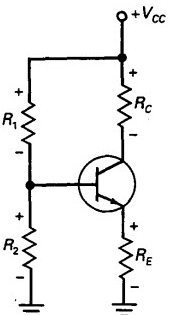
\includegraphics[scale=.5]{Imagenes/Polarizacion.png}
\end{figure}\\
Si queremos crear una analogía podría ser como un switch que está polarizado o no polarizado, on u off. Si lo polarizamos bien, [La razón por que tiene 4 resistencias la \textbf{Figura 1} es por que:] necesitamos que la tensión entre el colector y el emisor sea la mitad de la alimentación, en sintesis y palabras simples, las resistencias deben hacer que la tensión que pasará por el emisor y el colector deben ser igual a [$Vce = \frac{VCC}{2}$] en cuanto logramos esta condición tenemos un anplificador, está polarizado, lo encontramos en mitad de la recta de carga.\\
\vspace{1cm}
Otro concepto que debemos aprender es el punto \textbf{Q} que podriamos describirlo como el punto que se encuentran en los transistores para la polarización, para conseguirlo necesitamos que la tensión del colector y emisor sea la mitad del voltaje de entrada por ello en los transistores podemos encontrar Q1,Q2,Q3... como vemos en la siguiente imagen.\\
Definimos el punto Q como punto de quietud o Quiescent point [Punto de polarización]\\
\begin{figure}[hbtp]
\caption{PCB Con transistor}
\centering
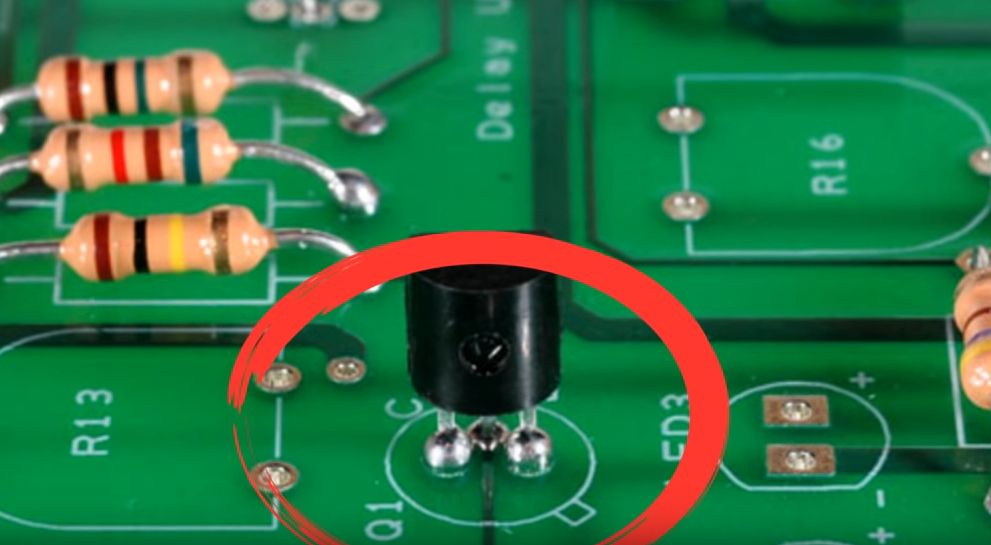
\includegraphics[scale=.3]{Imagenes/q1.png}\\
\end{figure}
\newpage

Cuando el voltaje que pasa por la patita de la base es mayor al que se le estaba aplicando en consancia decimos que la tensión que pasará por esa parte ser hace más grande, al igual pasa con su inversa, si una tension que tenemos constante en 3V le metemos una de 3.5 entonces veremos que el voltaje que se encuentra constante en la entrada sin llegar al tope de arriba o abajo en la recta se mantiene, habrá una variación al meter una amplitud mayor o menor, por lo que la onda del voltaje crecerá y de aqui podemos ver que si la corriente del pin base es mas pequeña, la corriente del pin emisor será mayor sin embargo, si metemos una corriente menor la corriente del pin emisor será menor. 
sin embargo la onda será de misma proporción a la original pero inversa en el eje de las 'y'
sin llegar a negativos[A menos que la armonía sea rota por un voltaje mayor al de los limites].\\
Los limites los podemos ver de manera que justifiquen VCE = Vcc/2 ya que nos posicionarán en la mitad de donde queremos comenzar nuestra onda.
\begin{figure}[hbtp]
\caption{onda amplificada}
\centering
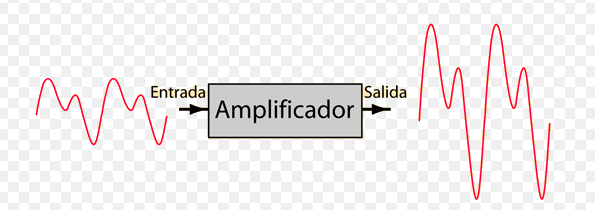
\includegraphics[scale=.6]{Imagenes/amp.png}\\
\end{figure}
para poder ver los pines emisor, colector y base debemos revisar los Datasheet de nuestro componente, como veremos en la siguiente imagen de un datasheet de un transistor 2n2222.\\
\newpage

\begin{figure}[hbtp]
\caption{De Alldatasheet}
\centering
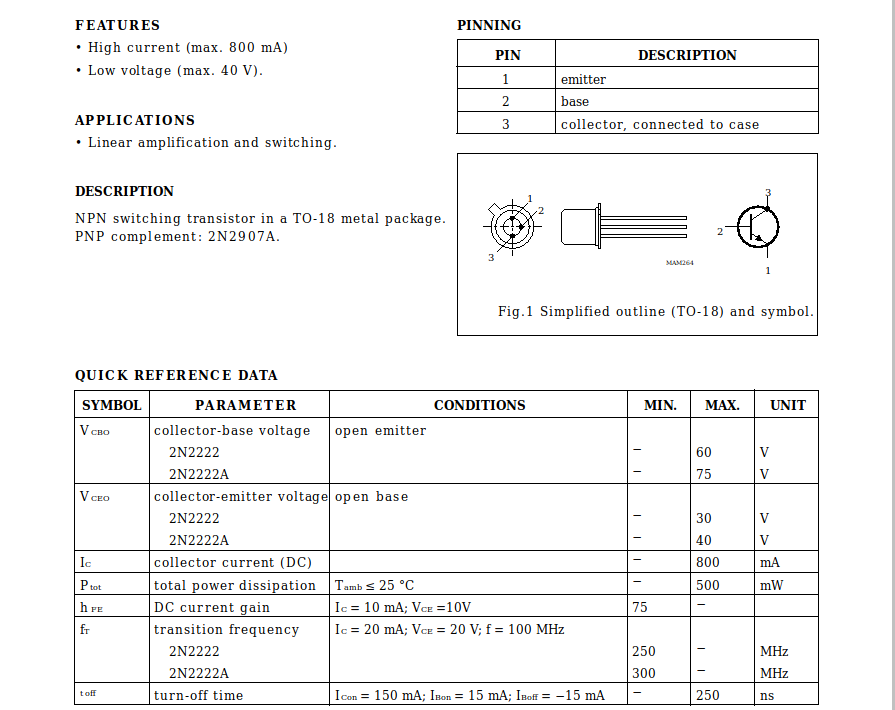
\includegraphics[scale=.5]{Imagenes/data.png}\\
\end{figure}
Antes teniamos transformadores que hacian la onda mas grande pero con base de una onda pequeñ, y le emitian de una cantidad determinada de su tamaño, aquí trabajaremos con voltajes un poco más altos y la onda será emitida a voltajes del doble de su tamaño.

\begin{huge}
\begin{center}
\textbf{Diferencias con amplificadores clase B}
\end{center}
\end{huge}
En vez de utilizar solo uno de los transistores en el clase B tenemos dos transistores que trabajan a la par para poder generar casi el mismo tipo de onda, por tanto se reduce, entre los dos amplifican y por tanto reducen la carga de trabajo de los transistores, como en una gondola, en vez de que reme uno, que remen dos.
por tanto la diferencia principal solo es que tienen 2 transistores que carga el trabajo uno de otro y la otra diferencia es con base a lo anterior, pues la onda no saldrá igual que si solo hubiese un transistor.
\newpage
Pero como tenemos una carga que funciona en positivo, veremos que el transistor numero dos, estará en los negativos, dependiendo del material del transistor será de donde comenzará la onda.


\begin{center}
\textbf{bibliografías}
\end{center}
Article
 J.I.Huircan AmpliÖcadores de Potencia Universidad de La Frontera, January 6, 2016


\end{large}
\end{document}